\documentclass[a4paper,12pt]{article} 
\usepackage[T2A]{fontenc}			
\usepackage[utf8]{inputenc}			
\usepackage[english,russian]{babel}	
\usepackage{amsmath,amsfonts,amssymb,amsthm,mathrsfs,mathtools} 
\usepackage{cancel}
\usepackage{hhline}
\usepackage{multirow}
\usepackage[colorlinks, linkcolor = purple, citecolor = purple]{hyperref}
\usepackage{upgreek}\usepackage[left=2cm,right=2cm,top=2cm,bottom=3cm,bindingoffset=0cm]{geometry}
\usepackage{tikz}
\usepackage{graphicx}
\usepackage{subfig}
\usepackage{titletoc}
\usepackage{pgfplots}
\usepackage{xcolor}
\usepackage{wrapfig}

\newcommand{\angstrom}{\text{\normalfont\AA}}
\author{Вихлянцев Константин, Цедрик Андрей\\
Группа Б01-109}
\title{5.10.1 Электронный парамагнитный резонанс.}
\date{}

%\begin{wrapfigure}{r}{0.5\textwidth}
%\begin{center}
%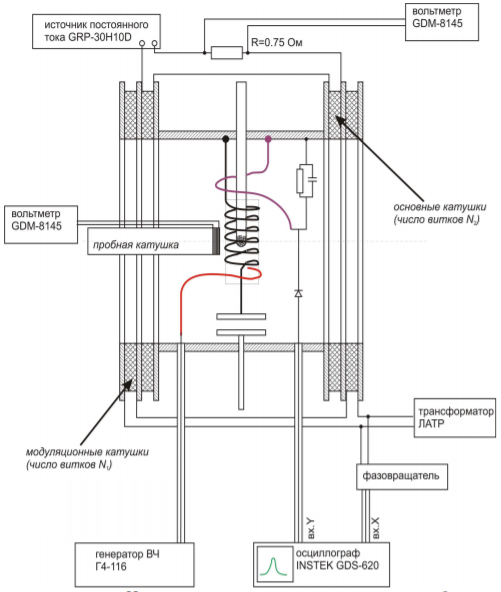
\includegraphics[width = 0.4\textwidth]{1.png}
%\end{center}
%\caption{}
%\end{wrapfigure}

%\begin{wrapfigure}{r}{0.5\textwidth}
%\begin{center}
%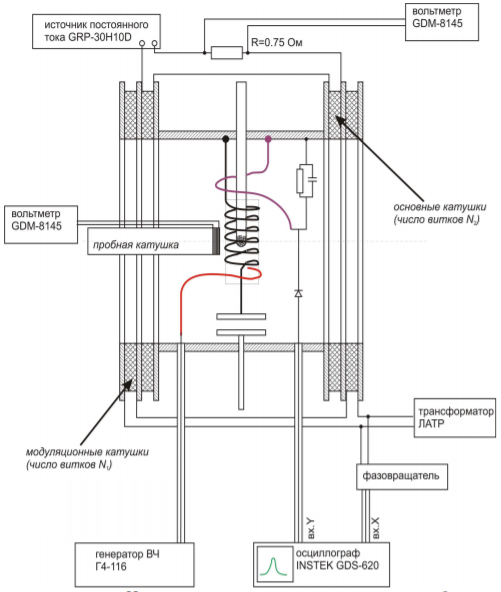
\includegraphics[width = 0.4\textwidth]{1.png}
%\end{center}
%\caption{}
%\end{wrapfigure}

\begin{document}
\maketitle
\textbf{В работе}: исследуется электронный парамагнитный резонанс (ЭПР) в молекуле дифенилпикрилгидразила (ДФПГ), определяется $g$-фактор электрона, измеряется ширина линий ЭПР.
\section*{Описание установки}
\begin{wrapfigure}{r}{0.4\textwidth}
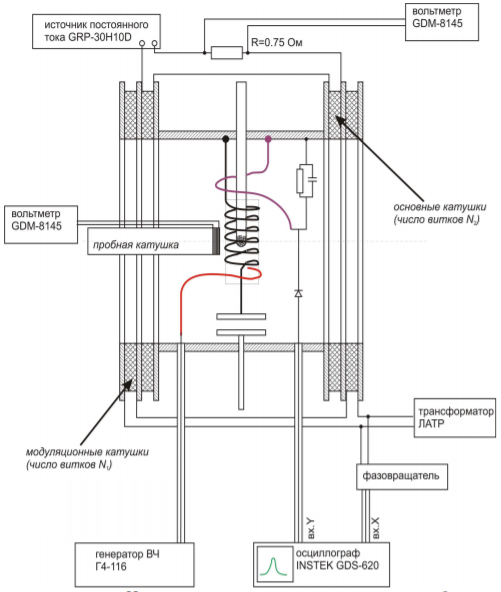
\includegraphics[width = 0.4\textwidth]{1.png}
\centering
\caption{Схема установки.}
\end{wrapfigure}
Схема установки представлена на Рис. 1. Образец (порошок ДФПГ) в стеклянной ампуле помещается внутрь катушки индуктивности, входящей в состав колебательного контура. Входящий в состав контура конденсатор состоит из двух пластин, разделённых воздушным зазором, одна из пластин может перемещаться поворотом штока. Колебания в контуре возбуждаются антенной, соединённой с генератором высокой частоты (ВЧ) Г4-116. Амплитуда колебаний поля в катушке индуктивности
измеряется по наводимой в петле связи ЭДС индукции. Высокочастотные колебания ЭДС
индукции в приёмном контуре детектируются диодом, измеряемая при помощи
осциллографа низкочастотная огибающая этого сигнала пропорциональна квадрату
амплитуды колебаний поля в катушке.\\
Постоянное магнитное поле создаётся пропусканием тока от источника постоянного тока через основные катушки. При этом при помощи вольтметра измеряется падение напряжения на резисторе в цепи основных катушек. Переменное поле небольшой амплитуды создаётся подачей на модуляционные катушки напряжения с регулируемого трансформатора ЛАТР. Для измерения амплитуды колебаний переменного поля используется пробная катушка известной геометрии, подключённая к вольтметру.\\
Характеристики катушек: пробная катушка $N_{\text{проб}} = 45$, $d_{\text{проб}} = 15.2\pm 0.1~\text{мм}$, основная катушка $N_{\text{осн}} = 6700$, $d_{\text{осн}} = 0.25\pm 0.01~\text{м}$,  модулирующая катушка $N_{\text{мод}} = 5000$, $d_{\text{мод}} = 0.30\pm 0.01~\text{м}$.
\section*{Ход работы и обработка данных}
\subsection*{Настройка ВЧ генератора.}
Для точной настройки генератора на резонансную частоту кантура спектроскопа, промодулируем высокочастотное колебание генератора низкой частотой. Установим частоту амплитудной модуляции 1 кГц и глубину модуляции 20\%. Меняя частоту генератора добъемся максимальной амплитуды колебаний на экране осцилогрофа. Зафиксируем полученное значение $f_0 = 162.2~\text{МГц}$.
\subsection*{Наблюдение сигнала резонансного поглощения.}
Подключим основные катушки к источнику постоянного тока, а модуляционные катушки к трансформатору ЛАТР. ВЧ-генератор переведём в режим непрерывной генерации, на канале осциллографа, подключённому к детектору, установим максимальную чувствительность. Подадим на модуляционные катушки напряжение $\sim 90~\text{В}$, и, плавно увеличивая постоянное напряжение на основных катушках, добиваемся возникновения на экране резонанстного поглощения. Добьёмся того, чтобы наблюдаемые пики были эквидистантны. Зафиксируем ток $I = 0.175 А \pm 0.001~\text{А}$.
\subsection*{Определение g-фактора.}
Для определения поля резонансного поглощения найдём связь между падением напряжения на резисторе в цепи основной катушки и магнитным полем. Для этого подадим в основные катушки переменный ток и измеряем при помощи пробной катушки
ЭДС индукции. \\
Переключим основные катушки на ЛАТР, переведём вольтметр, измеряющий
падение напряжения на резисторе $V_R$ в цепи основных катушек, в режим измерений на
переменном токе, установим ток через катушки, близкий к значению тока при наблюдении резонансного поглощения, измерим в этих условиях ЭДС индукции в пробных катушках. Для контроля однородности поля вносим катушку в центр магнита с передней $V_{\text{перед}} = 15.20 \pm 0.01 \text{ мВ}$ и задней $V_{\text{зад}} = 15.83 \pm 0.01 \text{ мВ}$
стороны установки. Тогда $V_{\text{сред}} = \left( V_{\text{перед}} + V_{\text{зад}}\right)/2 = 15.62 \pm 0.01 \text{ мВ}$. \\
Теперь мы можем посчитать индукцию основного магнитного поля по следующей формуле
\[V_{\text{сред}} = nB_0S\omega.\]
Следовательно,
\[B_0 = \dfrac{V_{\text{сред}}}{nS\omega} = 6.1 \pm 0.2~\text{мТл}.\]
Тогда, используя формулу $h \nu = g\mu_B B_{0}$, вычислим $g$-фактор электрона
\[g = \dfrac{hf_0}{\mu_B B_0} = 1.90 \pm 0.14.\]
Истинное значение $g$-фактора электрона $g = 2.0036$ лежит в пределах погрешности.
\subsection*{Определение ширины линии ЭПР.}
Для более точной настройки и определения ширины линии резонансного поглощения удобно подать на X-канал осциллографа напряжение, прикладываемое к модуляционным катушкам и наблюдать сигнал в XY-режиме. Фактически при этом на экране наблюдается зависимость поглощения в образце от приложенного переменного поля. Наблюдаемая картина симметрична относительно средней вертикальной оси. Из-за набегающей в электрической схеме расфазировки напряжений на экране наблюдаются два пика, соответствующие прохождению резонансного поглощения на растущем и падающем полупериодах модулирующего напряжения, поэтому пики совмещаем подстройкой фазовращателя.\\
Для определения ширины линии ЭПР определим по экрану осциллографа полный размах
модулирующего поля $A_{\text{полн}}$ и полную ширину кривой резонансного
поглощения на полувысоте $A_{\text{1/2}}$ . Не изменяя настроек, возьмём пробную катушку и внесём её внутрь соленоида максимально близко к образцу. Переменное поле модуляционных катушек наводит в пробной катушке ЭДС индукции $\mathcal{E}$, по которой можно определить величину поля. ЭДС индукции: $\mathcal{E} = 0.47\pm 0.04~\text{мВ}$. Размах и ширина кривой резонансного поглощения $A_{\text{полн}} = 3.8 \pm 0.2~\text{дел}$, $A_{\text{1/2}} = 1.6 \pm 0.2~\text{дел}$ (погрешность -- размер минимального деления осцилографа). Тогда амплитуда модулюрующего поля
\[B_{\text{мод}} = \dfrac{2\sqrt{2}\mathcal{E}}{\pi^2 d_{\text{проб}}^2 N_{\text{проб}}\nu} = 0.26 \pm 0.02~\text{мТл},\]
где $\nu = 50~\text{Гц}$ -- частота модулирующего напряжения. Полуширину на полувысоте линии резонансного поглощения посчитаем по формуле
\[\Delta B = \dfrac{A_{1/2}}{A_{\text{полн}}} B_{\text{мод}} = 0.109 \pm 0.014~\text{мТл}.\]
\begin{figure}[h]
    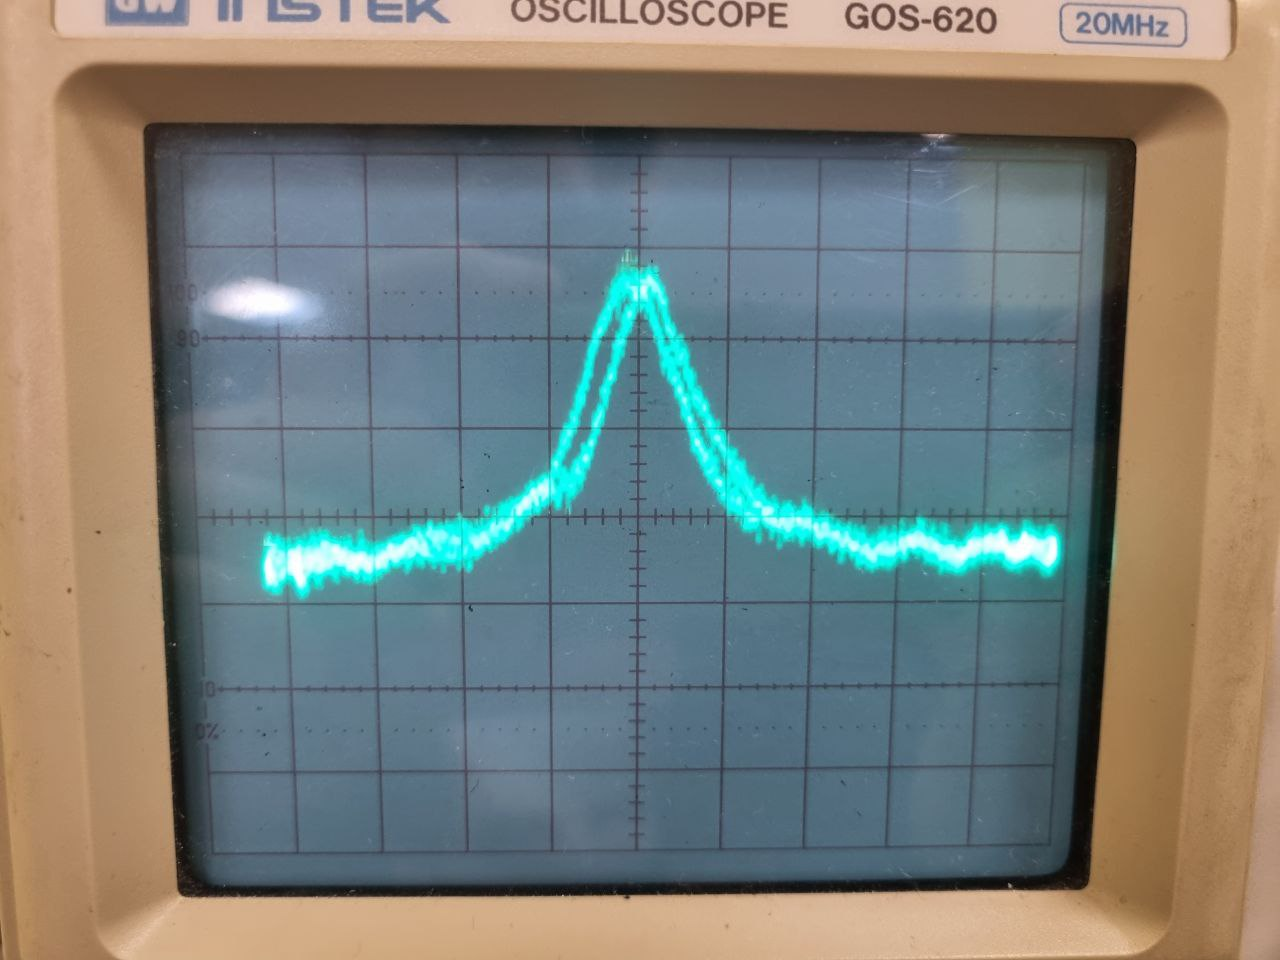
\includegraphics[scale=0.34]{hehe.jpg}
    \caption{Точная настройка резонансного поля}
    \centering
\end{figure} 
\section*{Заключение}
В данной работе был исследован ЭПР в молекуле ДФПГ, определен $g$-фактор электрона ${g = 1.90 \pm 0.14}$, а также измерена ширина линий ЭПР $\Delta B = 0.109 \pm 0.014~\text{мТл}$. Измеренный $g$-фактор электрона совпадает с табличным значением для свободного электрона: ${g_{free} = 2,0036}$. Это обусловлено тем, что ПР происходит на неспаренных электронах так же, как на свободных.
\end{document}

